%META {"question":"Đường thẳng d vuông góc với đoạn thẳng AB tại trung điểm M (AM = MB, có ký hiệu bằng nhau). Đường thẳng d là gì của đoạn thẳng AB?","options":["Đường trung trực của đoạn thẳng AB","Đường cao của một tam giác","Tia phân giác của một góc","Đường chéo của đoạn thẳng AB"],"answer":0,"note":"Đường thẳng vuông góc với đoạn thẳng tại trung điểm của nó gọi là đường trung trực của đoạn thẳng đó."}
\documentclass[border=5pt]{standalone}
\usepackage{tkz-euclide}
% Màu dùng chung cho toàn bộ hình vẽ (ảnh stack với nền tối của web)
\definecolor{tminc}{RGB}{226,232,240}   % chữ + nét chính
\definecolor{tmblue}{RGB}{0,210,255}    % nhấn neon xanh
\definecolor{tmpink}{RGB}{255,0,200}    % nhấn neon hồng
\definecolor{tmgreen}{RGB}{0,255,136}   % nhấn neon xanh lá
\color{tminc}

\begin{document}
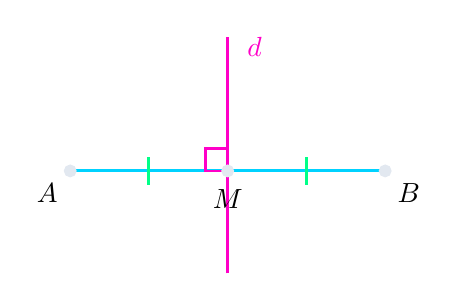
\begin{tikzpicture}[line width=1.1pt]
  \coordinate (A) at (0,0);
  \coordinate (B) at (4,0);
  \coordinate (M) at (2,0);
  \coordinate (U) at (2,-1.3);
  \coordinate (V) at (2,1.7);
  \draw[tmblue] (A) -- (B);
  \draw[tmpink] (U) -- (V);
  \tkzMarkRightAngles[size=0.28,color=tmpink,line width=1pt](A,M,V)
  \tkzMarkSegment[mark=|,color=tmgreen,size=5pt](A,M)
  \tkzMarkSegment[mark=|,color=tmgreen,size=5pt](M,B)
  \tkzDrawPoints[size=3.5,color=tminc,fill=tminc](A,B,M)
  \tkzLabelPoint[below left=1pt](A){$A$}
  \tkzLabelPoint[below right=1pt](B){$B$}
  \tkzLabelPoint[below=3pt](M){$M$}
  \node[tmpink] at (2.34,1.58) {$d$};
\end{tikzpicture}
\end{document}
